\documentclass[en]{university}

\faculty{Department of Computer Engineering}
\course{Computer Networks}
\subject{Homework 2}
\professor{Dr. Jafari}
\student{Parsa Mohammadian}

\begin{document}

\setupdocument

\section{}
\subsection{}
As we can see in the figure \ref{fig:WSProtocolStat}, UDP and TCP are used to transfer data over IPv4. Despite not all of the packets are used for loading \url{ce.sharif.edu}, browser had used both of them to transfer data. It used UDP for DNS queries and TCP for HTTP requests.

\begin{figure}
    \centering
    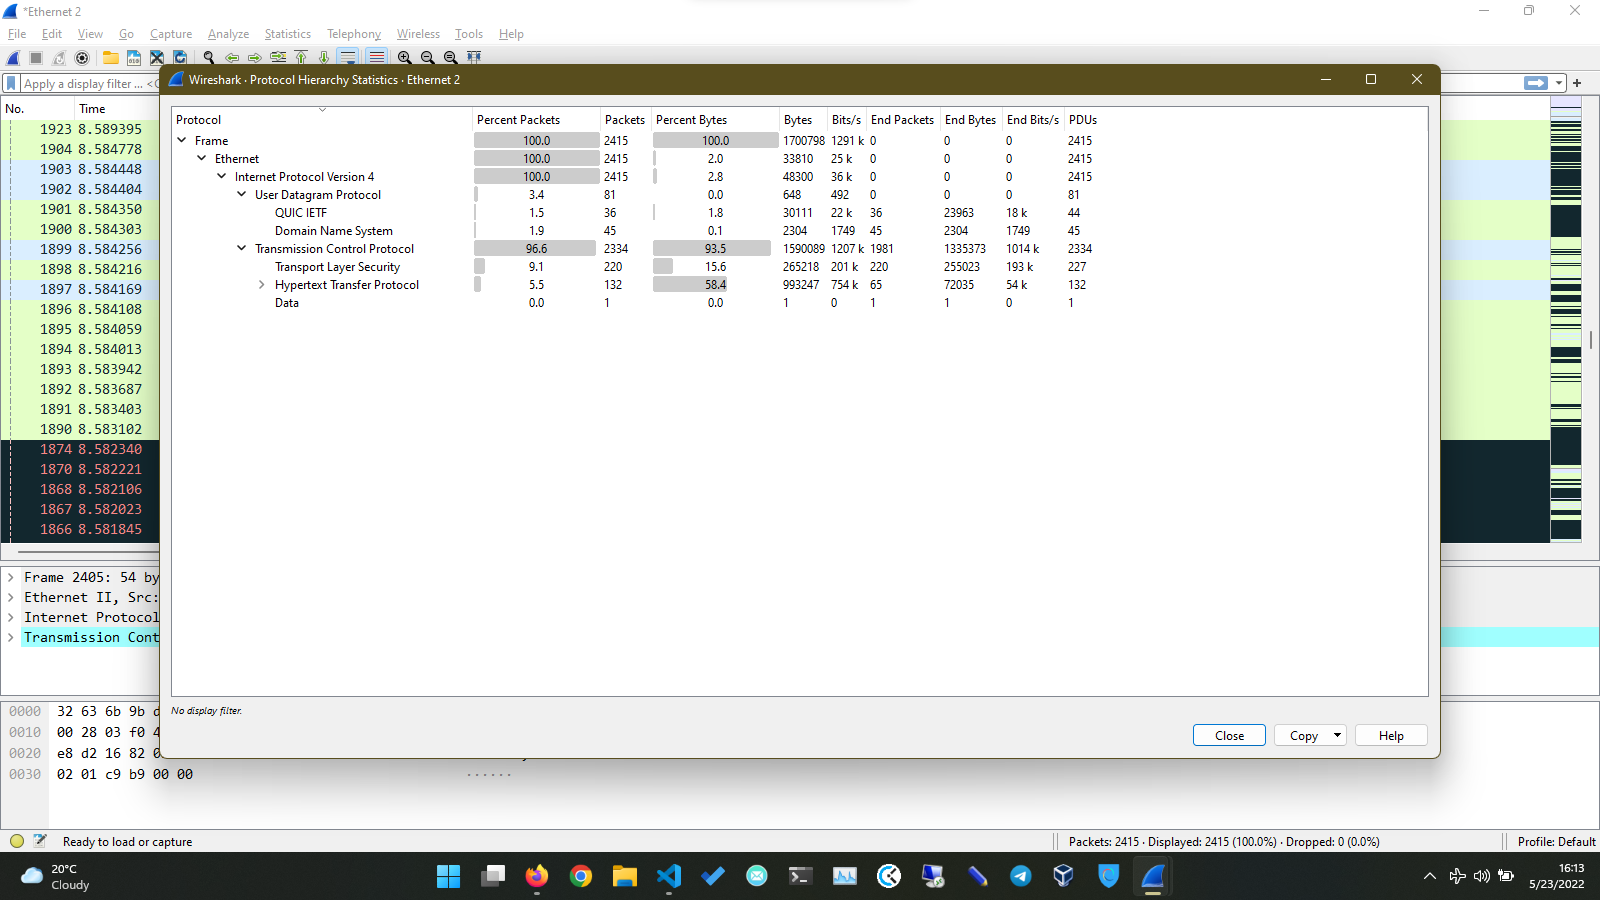
\includegraphics[width=\textwidth]{./resources/WSProtocolStat.png}
    \caption{Wireshark Protocol Statistics}
    \label{fig:WSProtocolStat}
\end{figure}

\subsection{}
First, we can sort the packets by the protocol type. Now we can see all of the DNS requests togehter. We can see the first DNS request for \url{ce.sharif.edu} in the figure \ref{fig:WSDNS}. As we can see, the first request is sent from \url{172.20.10.3} to \url{192.168.250.250} for A record of \url{ce.sharif.edu}. Both of these IP addresses are private LAN addresses so this request is probably to a local DNS. After that we have the second packet sent from \url{172.20.10.3} to \url{8.8.8.8} which is the Google DNS server. Then Google DNS server responds and sends the \url{81.31.168.124} as the IP address of \url{ce.sharif.edu}. After that we have exact same packets sent and received but for AAAA record; and the final response is not IP address but it is SOA record (\url{ns1.sharif.ir}) which is a record that tells the server where to find other records. After that we can see some other DNS request, like those for \url{ce.sharif.edu}, for subdomains of \url{ce.sharif.edu} which are hardware, ai, it, and web. 

\begin{figure}
    \centering
    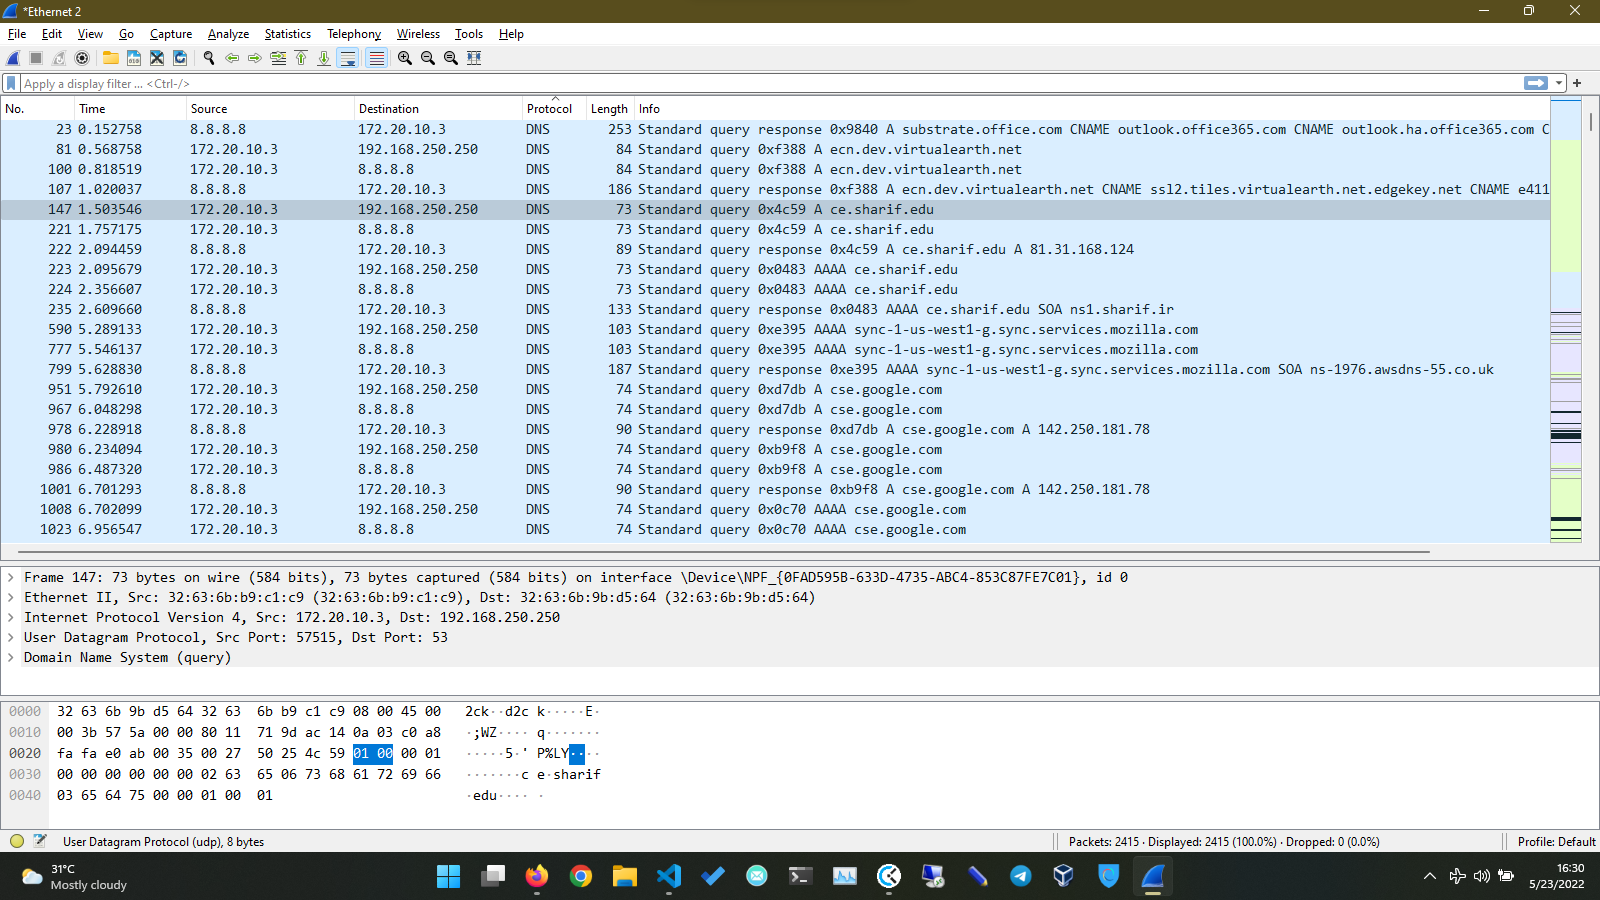
\includegraphics[width=\textwidth]{./resources/WSDNS.png}
    \caption{DNS Requests}
    \label{fig:WSDNS}
\end{figure}

\section{}
RTMP or Real-Time Messaging Protocol is a protocol for streaming media over the Internet. It was primarily developed by Micromedia (which is now owned by Adobe Systems) and is used by Adobe Flash Media Server (FMS) to stream media to the client. 

RTMP is used in transport-layer protocol like TCP and UDP.

The structure of RTMP packet is shown in the figure \ref{fig:RTMPPacket}. 

\begin{figure}
    \centering
    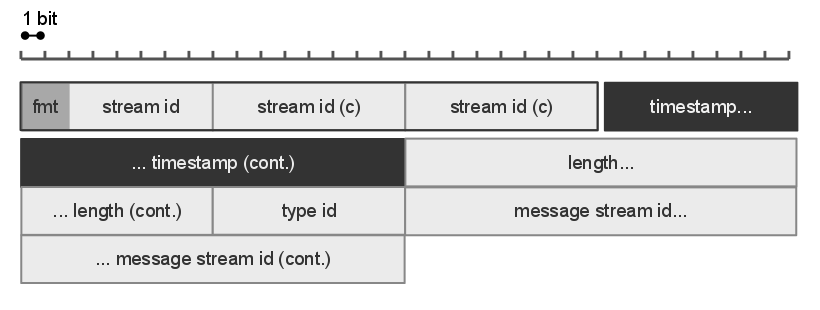
\includegraphics[width=0.5\textwidth]{./resources/RTMPPacket.png}
    \caption{RTMP Packet Structure}
    \label{fig:RTMPPacket}
\end{figure}

The handshake process is shown in the figure \ref{fig:RTMPHandshake}.

\begin{figure}
    \centering
    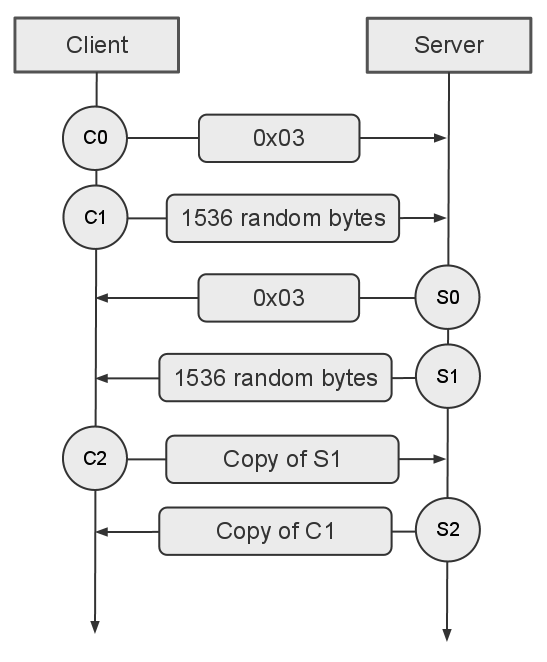
\includegraphics[width=0.5\textwidth]{./resources/RTMPHandshake.png}
    \caption{RTMP Handshake Diagram}
    \label{fig:RTMPHandshake}
\end{figure}

\end{document}